\section{Zielsetzung}
In diesem Versuch soll die Funktionsweise einer Wärmepumpe untersucht werden.

\section{Theorie}
Der zweite Hauptsatz der Thermodynamik sagt aus, dass Wärmeenergie immer von einem wärmeren zu einerm kälteren Medium übergeht, wenn
keine weitere Arbeit aufgewendet wird. Die Wärmepumpe wirkt diesem entgegen, sie bewirkt also, dass Wärmeenergie von einem kälteren zu einem
wärmeren Medium übergeht, indem sie diese mechanische Arbeit verrichtet.

Durch den 1. Hauptsatz der Themodynamik kann man folgenden Beziehung für die an das wärmere Medium abgegebene Wärmemenge $Q_1$, die aufgenommene
Wärmemenge aus dem kälteren Medium $Q_2$  und die verrichtete Arbeit $A$ herstellen

\begin{equation*}
  \label{eq:1}
  Q_1 = Q_2 + A \, .
\end{equation*}

Durch einer Vorraussetzung, dass der Vorgang der Wärmetransport reversible sein muss, also dass es ohne Verluste wieder rückgängig gemacht
werden kann, lässt sich aus dem 2. Hauptsatz der Thermodynamik eine weitere Gleichung zwischen den Wärmemengen $Q_1$ und $Q_2$ und deren
Temperaturen $T_1$ und $T_2$ aufstellen.

\begin{equation}
  \label{eq:2}
  \frac{Q_1}{T_1} - \frac{Q_2}{T_2} = 0.
\end{equation}

Da diese Vorraussetzung eines reversiblen Wärmetransportes aber technisch nicht umsetzbar ist, gilt für den realen Fall

\begin{equation}
  \label{eq:3}
  \frac{Q_1}{T_1} - \frac{Q_2}{T_2} > 0.
\end{equation}

Die Güteziffer $\nu$ einer realen Wärmepumpe, welche das Verhältnis zwischen der aufgewendeten Arbeit und der an das wärmere Medium abgegebenen Wärmemenge beschreibt,
ist wie folgt definiert

\begin{equation}
  \label{eq:4}
  \nu = \frac{Q_1}{A} < \frac{T_1}{T_1 -T_2}\, .
\end{equation}

\subsection{Funktionsweise einer Wärmepumpe}

\begin{figure}
  \centering
  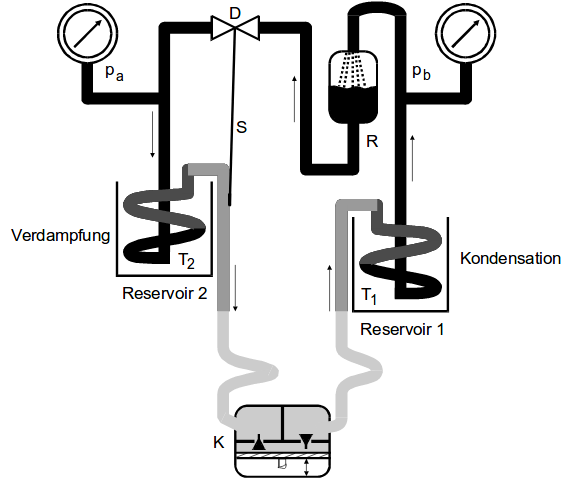
\includegraphics[scale = 0.4]{SchematischerAufbau.png}
  \caption{Schematischer Aufbau einer Wärmepumpe. \cite{Quelle}}
  \label{Abb:1}
\end{figure}

In Abbildung \ref{Abb:1} ist der schematische Aufbau dargestellt.
Zum Wärmetransport wird bei der Wärmepumpe ein reales Gas verwendet, welches bei dem Verdampfen Wärme aufnimmt und bei der Verflüssigung
Wärme abgibt. Dieses Gas durchläuft sowohl beide Reservoire als auch das Drosselventil.
Wenn das Gas an zum Reservoir 2 gelangt, ist dieses flüssig und verdampft beim Durchströmen dieses Reserviors durch die Druckdifferenz und
entzieht dem Reservoir 2 somit die Verdampfungswärme. Das verdampfte Gas durchströmt nun das Reseroir 1 und wird dort durch die Druckdifferenz wieder verflüssigt,
es gibt also die Verdampfungswärme an das Reservoir 1 ab. Das Druckventil D sorgt dabei für die Druckdifferenz und der Kompressor K für die
Bewegung des Kreislaufes.
Weiterhin gibt es noch einige Bauelemente, die aber zu eigentlichen Funktionsweise einer Wärmepumpe nicht beitragen. So wird noch ein Reiniger vor
dem Kompressor installiert, sodass die Gasbläschen aus dem flüssigen Medium herausgefiltert werden.

\subsection{Berechnung der Kenngrößen einer Wärmepumpe}
In diesem Versuch werden einige Kenngrößen dieser Wärmepumpe berechnet.
Zunächst die schon oben beschriebene reale \textbf{Güteziffer}, diese kann durch die Messreihe in diesem Versuch wie folgt bestimmt werden

\begin{equation}
  \label{Güteziffer}
    \nu = \frac{\increment Q_1}{\increment t N},
\end{equation}

mit

\begin{equation}
  \label{Güteziffer2}
  \frac{\increment Q_1}{\increment t} = (m_1c_w + m_kc_k) \frac{\increment T_1}{\increment t},
\end{equation}

wobei $m_1 c_w$ die Wärmekapazität des Wasser aus Reservoir 1 und $m_k c_k$ die Wärmekapazität der Kupferschlange und des Eimers beschreibt.

Eine weitere Kenngröße ist der \textbf{Massendurchsatz $ \frac{\increment m}{\increment t}$ }, dieser kann durch $T_2$ und die Verdampfungswärme $L$ berechnet werden mit
 \begin{equation}
   \label{Massendurchsatz1}
   \frac{\increment Q_2}{\increment t} = (m_2 c_W + m_k c_k) \frac{\increment T_2}{\increment t}
 \end{equation}
und
\begin{equation}
  \label{Massendurchsatz2}
  \frac{\increment Q_2}{\increment t} = L \frac{\increment m}{\increment t} .
\end{equation}

Zur Berechnung der \textbf{Mechanischen Kompressorleitung $N$} wird folgende Formel verwendet

\begin{equation}
  \label{Leistung}
  N_{mech} = \frac{\increment A_m}{\increment t} =  \frac{1}{\kappa - 1} \left( p_b \sqrt[\kappa]{\frac{p_a}{p_b}} - p_a \right) \frac{1}{\rho} \frac{\increment m}{\increment t},
\end{equation}

wobei $\rho$ die Dichte des gasförmigen Mediums und $\kappa$ das Verhältnis der Molwärmen $C_p$ und $C_v$ ($\kappa>0$) beschreibt.
Die Differenzenquotienten lassen sich auch die Differentialquotienten ersetzen.

\section{Durchführung}

\begin{figure}
\centering
  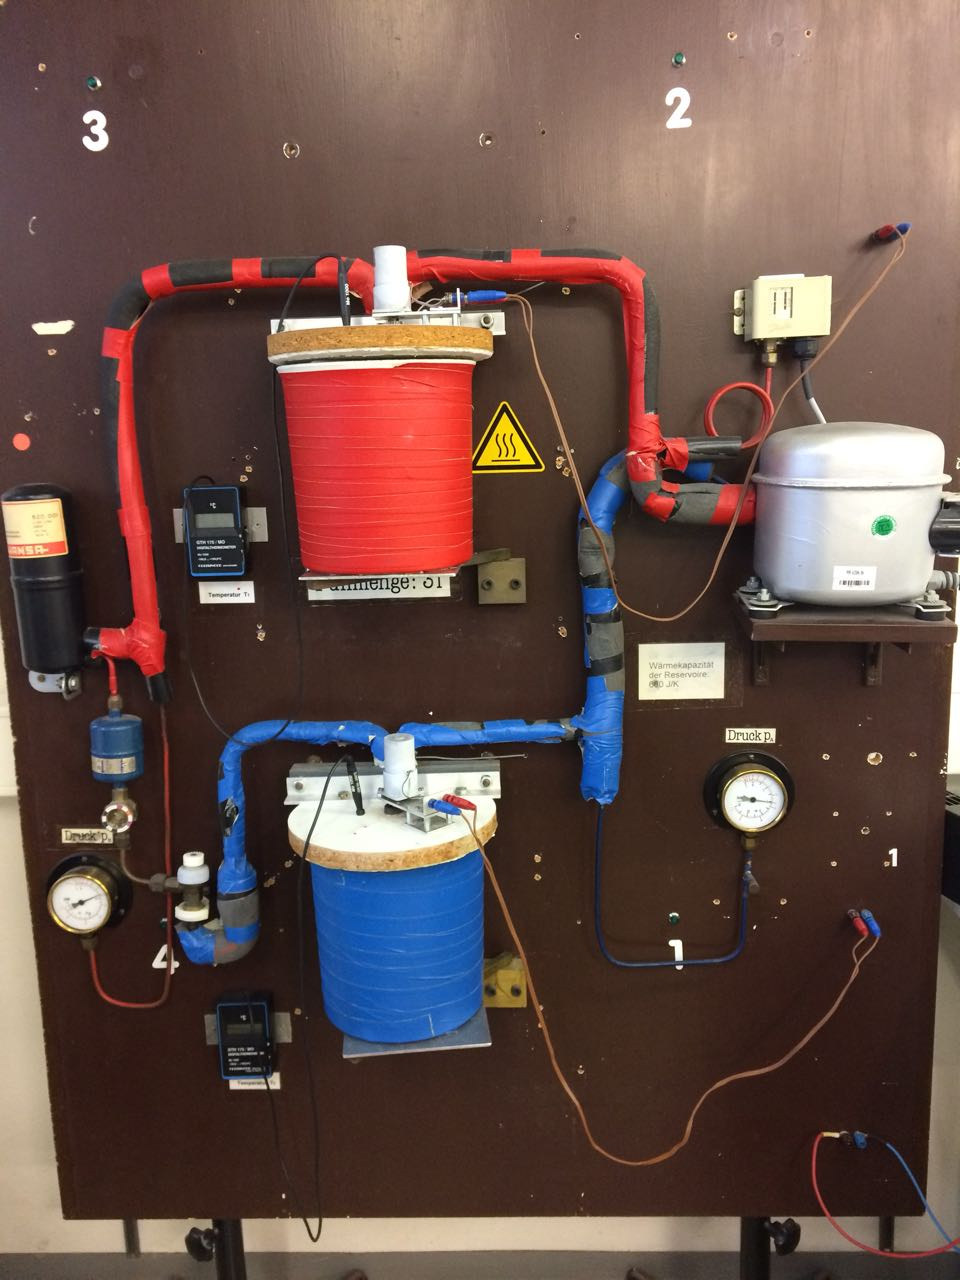
\includegraphics[scale = 0.2]{Aufbau.jpeg}
  \caption{Versuchsaufbau}
  \label{Abb:2}
\end{figure}
Zu Beginn werden die zwei Behälter (siehe Abbildung \ref{Abb:2}) mit je 4 Litern Wasser befüllt. Zu überprüfen ist zunächst, ob die Rührmotoren
in den Behältern einwandfrei funktionieren, um eine möglichst homogene Mischung des Wassers zu erhalten.
Die Messung wird gestartet, sobald die Wärmepumpe läuft. Jede Minute werden sowohl die Drücke $p_a$ und $p_b$, als auch die Temperaturen $T_1$ und
$T_2$ abgelesen. Außerdem wird zusätzlich noch die Leistungsaufnahme des Kompressors notiert. Die Messreihe wird gestoppt, wenn
$T_1$ die \SI{50}{\celsius} erreicht.

\section{Auswertung}
\subsection{Temperaturverläufe}
In Tabelle \ref{tab1} sind die im Wärme- beziehungsweise Kältereservoir gemessenen Temperaturen
$\text{T}_1$ und $\text{T}_2$ mit den zugehörigen Drücken $\text{P}_1$ und $\text{P}_2$, sowie
die generierte Leistung der Wärmepumpe aufgelistet. Zu den Drücken $\text{P}_1$ und $\text{P}_2$
wurde bereits ein bar Atmosphärendruck dazuaddiert.
\FloatBarrier
\begin{table}
  \centering
  \caption{Messwerte zur Erstellung der Plots}
  \label{tab1}
  \begin{tabular}{ c c c c c c }
    \toprule
    {t / s} & {$T_1$ / $\si{\celsius}$} & {$T_2$ / $\si{\celsius}$} & {$P_1$ / bar} & {$P_2$ / bar} & {P / W} \\
    \midrule
     0  &   20.3   &   20.4  &  5.1  &  8.00   &  210  \\
    60  &   21.3   &   20.4  &  2.4  &  7.75   &  160  \\
   120  &   22.1   &   20.3  &  2.7  &  7.00   &  175  \\
   180  &   23.4   &   19.4  &  2.9  &  7.50   &  185  \\
   240  &   25.1   &   17.9  &  3.0  &  7.75   &  195  \\
   300  &   27.0   &   16.0  &  3.1  &  8.00   &  200  \\
   360  &   29.0   &   14.1  &  3.2  &  8.50   &  203  \\
   420  &   31.0   &   12.3  &  3.2  &  9.00   &  205  \\
   480  &   33.0   &   10.5  &  3.2  &  9.50   &  206  \\
   540  &   34.9   &    8.6  &  3.1  &  9.75   &  206  \\
   600  &   36.7   &    6.8  &  3.2  &  10.25  &  210  \\
   660  &   38.5   &    5.2  &  3.2  &  10.50  &  211  \\
   720  &   40.2   &    3.6  &  3.2  &  11.00  &  215  \\
   780  &   41.9   &    2.2  &  3.2  &  11.50  &  215  \\
   840  &   43.5   &    1.2  &  3.2  &  11.75  &  215  \\
   900  &   45.1   &    0.4  &  3.2  &  12.00  &  213  \\
   960  &   46.5   &    0.0  &  3.2  &  12.50  &  210  \\
   1020 &   48.0   &   -0.6  &  3.2  &  12.75  &  207  \\
   1080 &   49.1   &   -1.0  &  3.1  &  13.00  &  205  \\
   1140 &   50.3   &   -1.4  &  3.1  &  13.50  &  205  \\
   \bottomrule
 \end{tabular}
\end{table}

Der Temperaturverlauf in den beiden Reservoirs ist in Abbildung \ref{abb1} zu sehen.
Die eingezeichnete Ausgleichsfunktion der beiden Temperaturverläufe wird mittels der Funktion
\FloatBarrier
\begin{align*}
  T(t) = \text{A} t^2 + \text{B} t + \text{C}
\end{align*}
beschrieben.
\begin{figure}
  \centering
  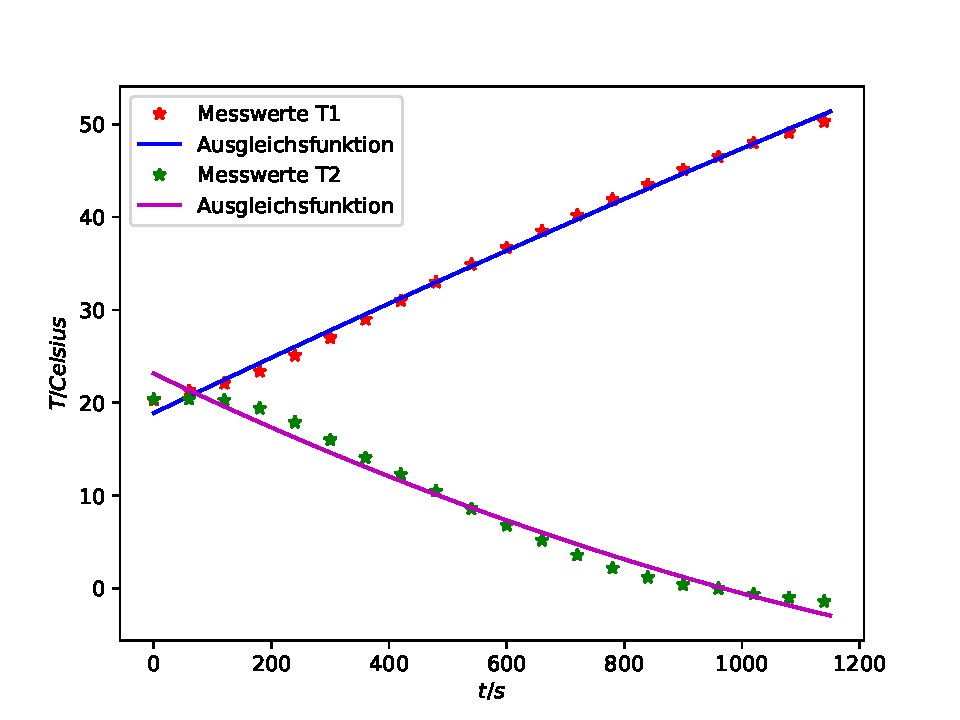
\includegraphics[scale=0.7]{plota.pdf}
  \caption{Temperaturverläufe in den Reservoirs gegen die Zeit aufgetragen}
  \label{abb1}
\end{figure}

Die Koeffizienten für das Wärmereservoir werden mit Hilfe des Programms scipy.optimize ermittelt und betragen:
\begin{align*}
  \symup{A_1} &= \SI{-1.7(14)}{\mu \kelvin \per \second \square}\\
  \symup{B_1} &= \SI{0.0302(16)}{\kelvin \per \second}\\
  \symup{C_1} &= \SI{292.05(40)}{\kelvin}\\
\end{align*}

\noindent Die Koeffizienten für das Kältereservoir betragen:
\begin{align*}
  \symup{A_2} &= \SI{6.7(14)}{\mu \kelvin \per \second \square}\\
  \symup{B_2} &= \SI{0.0303(31)}{\kelvin \per \second}\\
  \symup{C_2} &= \SI{296.25(27355)}{\kelvin}\\
\end{align*}

\noindent In Tabelle \ref{tab2} sind die Differenzenquotienten $f = \frac{\partial T}{\partial t}$ für die beiden Reservoirs,
die nach folgender Formel berechnet wurden:
\begin{align*}
  \frac{\Delta T}{\Delta t} = \symup{A} t + \symup{B},
\end{align*}
zu sehen.
\FloatBarrier
\begin{table}
  \centering
  \caption{Differenzenquotienten des Wärme- und Kältereservoirs}
  \label{tab2}
  \begin{tabular}{ c c c }
    \toprule
    {$t$ / $\si{\second}$} & {$\frac{\Delta T_1}{\Delta t}$ / $\si{\kelvin \per \second}$} & {$\frac{\Delta T_2}{\Delta t}$ / $\si{\kelvin \per \second}$}\\
    \midrule
  120 & 0,0300 \pm 0.0016  &  0,0295 \pm 0,0031  \\
  240 & 0.0298 \pm 0.0016  &  0,0287 \pm 0,0031  \\
  480 & 0.0294 \pm 0.0017  &  0,0271 \pm 0,0032  \\
  960 & 0.0210 \pm 0.0021  &  0,0239 \pm 0,0034  \\
   \bottomrule
  \end{tabular}
\end{table}

\noindent Der Fehler für den Diffenrenzenquotienten wird mit Hilfe der Gaußschen Fehlerfortpflanzung
berechnet, da in dessen Berechnung zwei fehlerbehaftete Größen A und B auftauchen:
\begin{align*}
  \Delta f = \sqrt{(\symup{A} \cdot \Delta \symup{A})^2 + \Delta \symup{B}^2}
\end{align*}
\FloatBarrier

\subsection{Güteziffer}
\noindent Im Anschluss daran wird mittels der Formel:
\begin{align*}
  \nu_\symup{real} = \frac{1}{\symup{P}} (m_1 c_\text{w} + m_\symup{k} c_\symup{k})\frac{\Delta T_1}{\Delta t}
\end{align*}
die reale Güteziffer der im Experiment verwendeten Wärmepumpe berechnet und mit dem Theoriewert
für die ideale Güteziffer verglichen, der sich aus folgender Gleichung ergibt:
\begin{align*}
  \nu_\symup{ideal} = \frac{T_1}{(T_1-T_2)} .
\end{align*}
Der Wert $\text{c}_\text{k} \text{m}_\text{k}$ ist dabei mit $\SI{660}{\joule \per \kelvin}$ die
spezifische Wärmekapazität der verwendeten Apparatur. Die Masse des Wassers $\text{m}_1$ beträgt
in diesem Fall $\SI{3}{\kilo \gram}$ und dessen spezifische Wärmekapazität $c_\symup{w}$ beträgt
$\SI{4183}{\joule \per \kelvin}$ \cite{Q1}. Die Leistung der Wärmepumpe ist für die verschiedenen Zeiten
unterschiedlich und ist ebenfalls zusammen mit den Ergebnissen in \ref{tab3} angegeben:

\begin{table}
  \centering
  \caption{Ideale und reale Güteziffer der Wärmepumpe im Vergleich}
  \label{tab3}
  \begin{tabular}{c c c c c}
    \toprule
    {$t$ / s} & { P / W} & {$\nu_\symup{ideal}$} & {$\nu_\symup{real}$} & {Abweichung / $\%$ }\\
    \midrule
    120 & 175 & 12,27 & $2,26 \pm 0,12$ &  81,51\\
    240 & 195 &  3,49 & $2,02 \pm 0,11$ &  42,12\\
    480 & 206 &  1,46 & $1,88 \pm 0,11$ &  28,76\\
    960 & 210 &  0,99 & $1,80 \pm 0,13$ &  81,82\\
    \bottomrule
  \end{tabular}
\end{table}

\subsection{Massendurchsatz}
Der Massendurchsatz lässt sich mit folgender Formel berechnen:
\begin{align*}
  (m_2 c_\symup{w} + m_\symup{k} c_\symup{k}) \frac{\Delta T_2}{\Delta t} = L \frac{\Delta m}{\Delta t} .
\end{align*}
Um dies zu berechnen, muss zunächst die Verdampfungswärme L des Transportgases Dichloridfluormethan
bestimmt werden. Dies geschieht, indem eine lineare Ausgleichsrechnung durchgeführt wird:
\begin{align*}
  ln(P_1) = \symup{a} \frac{1}{T_1} + \symup{b}
\end{align*}
Der Logarithmus von $P_1$ wird dann gegen die Temperatur aufgetragen, was in Abbildung \ref{abb2} zu sehen ist.
Für a ergibt sich dann ein Wert von $2180 \pm 90$
\FloatBarrier
\begin{figure}
  \centering
  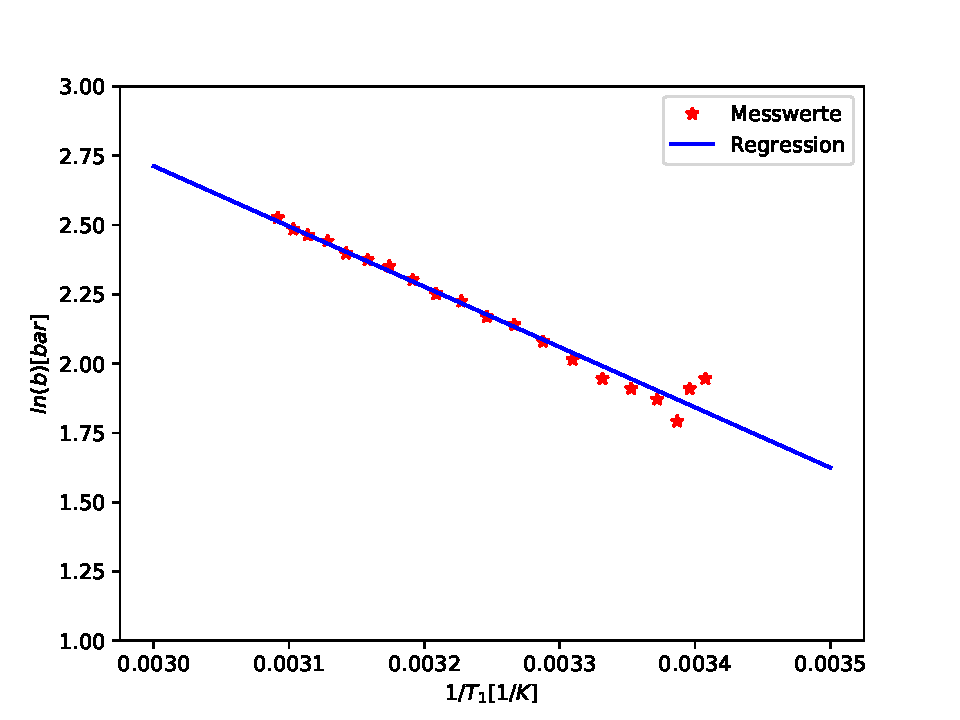
\includegraphics[scale=0.7]{plotb.pdf}
  \caption{Lineare Regression zur Bestimmung von L}
  \label{abb2}
\end{figure}

\noindent Mit diesem Wert a lässt sich dann L berechnen :
\begin{align*}
  L = -\symup{a} \symup{R}
\end{align*}
R ist die ideale Gaskonstante mit $\SI{8.314}{\joule \per \mol}$ \cite{Dem}.
So ergbit sich ein Wert für $L$ :
\begin{align*}
  L = \SI{18.1(7)}{\kilo \joule \per \mol}
\end{align*}
Die molare Masse von Dichloridfluormethan beträgt $\SI{120,91}{\gram \per \mol}$ \cite{Q1},
woraus sich für $L$ folgender Wert ergibt:$ L = \SI{150(6)}{\joule \per \gram}$.
Der Fehler für die Verdampfungswärme errechnet sich mit der Formel:
\begin{align*}
  \Delta L = -R \Delta \symup{a} .
\end{align*}
\FloatBarrier

Der Massendurchsatz $g$ lässt sich dann einfach berechnen, wobei sich der Fehler hierfür
aus folgender Formel berechnet:
\begin{align*}
  \Delta g = \sqrt{\left((m_2 c_\symup{w} + m_\symup{k} c_\symup{k}) \frac{\Delta T_2}{L^2 \Delta t} \Delta L\right)^2 + \left(\frac{(m_2 c_\symup{w} + m_\symup{k} c_\symup{k})}{L} \Delta \left(\frac{\Delta T_2}{\Delta t}\right) \right)^2}
\end{align*}
Hierbei beträgt $m_2$ wie $m_1$ $\SI{3}{\kilo \gram}$.
\FloatBarrier
\begin{table}
  \centering
  \caption{Massendurchsatz der Wärmepumpe zu verschiedenen Zeiten}
  \label{tab4}
  \begin{tabular}{ c c }
    \toprule
    {$t$ / $s$} & {$\frac{\Delta m}{\Delta t}$ / $\si{\gram \per \second}$} \\
    \midrule
    120   &   2,60 \pm 0,29  \\
    240   &   2,53 \pm 0,29  \\
    480   &   2,39 \pm 0,30  \\
    960   &   2,10 \pm 0,31  \\
    \bottomrule
  \end{tabular}
\end{table}



\subsection{Mechanische Kompressorleistung}
Zur Bestimmung der mechanischen Kompressorleistung:
\FloatBarrier
\begin{align*}
  \symup{N}_\symup{mech} = \frac{1}{\kappa-1}\left(\symup{P}_2 \sqrt[\kappa]{\frac{\symup{P}_1}{\symup{P}_2}}-\symup{P}_1)\right)\frac{1}{\rho} \frac{\Delta m}{\Delta t} ,
\end{align*}
muss zunächst $\rho$ bestimmt werden. Dies geschieht mit Hilfe folgender Formel:
\begin{align*}
  \rho = \frac{\rho_0 \symup{P}_1 \symup{T}_0}{\symup{p}_0 \symup{T}_2} .
\end{align*}
Hierbei ist $\rho_0 = \SI{5,51}{\gram \per \litre}$, $\symup{T} = \SI{273,15}{\kelvin}$, $p = \SI{1}{\bar}$ und $\kappa = 1,14$ in der Versuchsanleitung angegeben.
Der Fehler für die mechanische Kompressorleistung, der sich aus der weiteren Berechnung mit Hilfe des fehlerbehaftetetn Massendurchsatzes ergibt,
wird mit Hilfe folgender Formel berechnet:
\begin{align*}
  \Delta  N = \frac{1}{\kappa - 1} \left( \symup{P}_2 \sqrt[\kappa]{\frac{\symup{P}_1}{\symup{P}_2}} - \symup{P}_1 \right) \frac{1}{\rho} \cdot \Delta \left(\frac{\Delta m}{\Delta t}\right)
\end{align*}

\begin{table}
  \centering
  \caption{Mechanische Kompressorleistung}
  \label{tab5}
  \begin{tabular}{ c c c }
    \toprule
    {$t$ / $s$} & {$\rho$ / $\si{\kilo \gram \per m^3}$}  &  {$\symup{N}_\symup{mech}$ / $\si{\watt}$} \\
    \midrule
    120   &   13,85   &   $4,5 \pm 0,5$\\
    240   &   15.51   &   $4,3 \pm 0,5$\\
    480   &   16.98   &   $4,6 \pm 0,6$\\
    960   &   17.63   &   $5,0 \pm 0,7$\\
    \bottomrule
  \end{tabular}
\end{table}

\section{Diskussion}
Beim Vergleich der realen mit der idealen Güteziffer fallen sofort große Abweichungen auf. Diese sind eventuell
durch eine nicht ausreichende Isolierung der beiden Reservoirs und der Wärmeleitungen zu erklären.
Des Weiteren wurde das Abfüllen der Wassermengen für die Reservoirs lediglich ein einfacher
Kolben mit einer Markierung verwendet und die Menge wurde im Anschluss nicht exakt vermessen,
weshalb in der Auswertung immer von exakt drei Kilogramm Wassermenge ausgegangen wurde. Um hier
genauer vorzugehen, müsste die Wassermenge, die sich in den beiden Behältern befindet, exakt bestimmt werden.
Eine weitere Fehlerquelle bei der Durchführung des Versuchs besteht darin, dass es nicht möglich ist alle vier
Messdaten simultan von den weit auseinanderliegenden Messuhren abzulesen.
Ebenfalls ist nicht davon auszugehen, dass es sich es bei dem in der verwendeten Wärmepumpe befindlichen Gases um
ein ideales Gas handelt. Des weiteren erfolgt die Kompression des Gases keinesfalls adiabatisch, was bedeutet,
dass davon auszugehen ist, dass es im Innern der Leitungen zu Reibung kommt, die wiederum zu einem irreversiblen
Wärmeverlust führen. Die ebenfalls sehr geringe mechanische Kompressorleistung könnte ein weiteres Indiz dafür sein,
dass es im Innern der Leitungen zu Reibungsverlusten kommt, weshalb nicht die gesamte Leistung in der Wärmepumpe
umgewandelt wird.


\nocite{*}
\printbibliography
